\begin{figure}
\centering
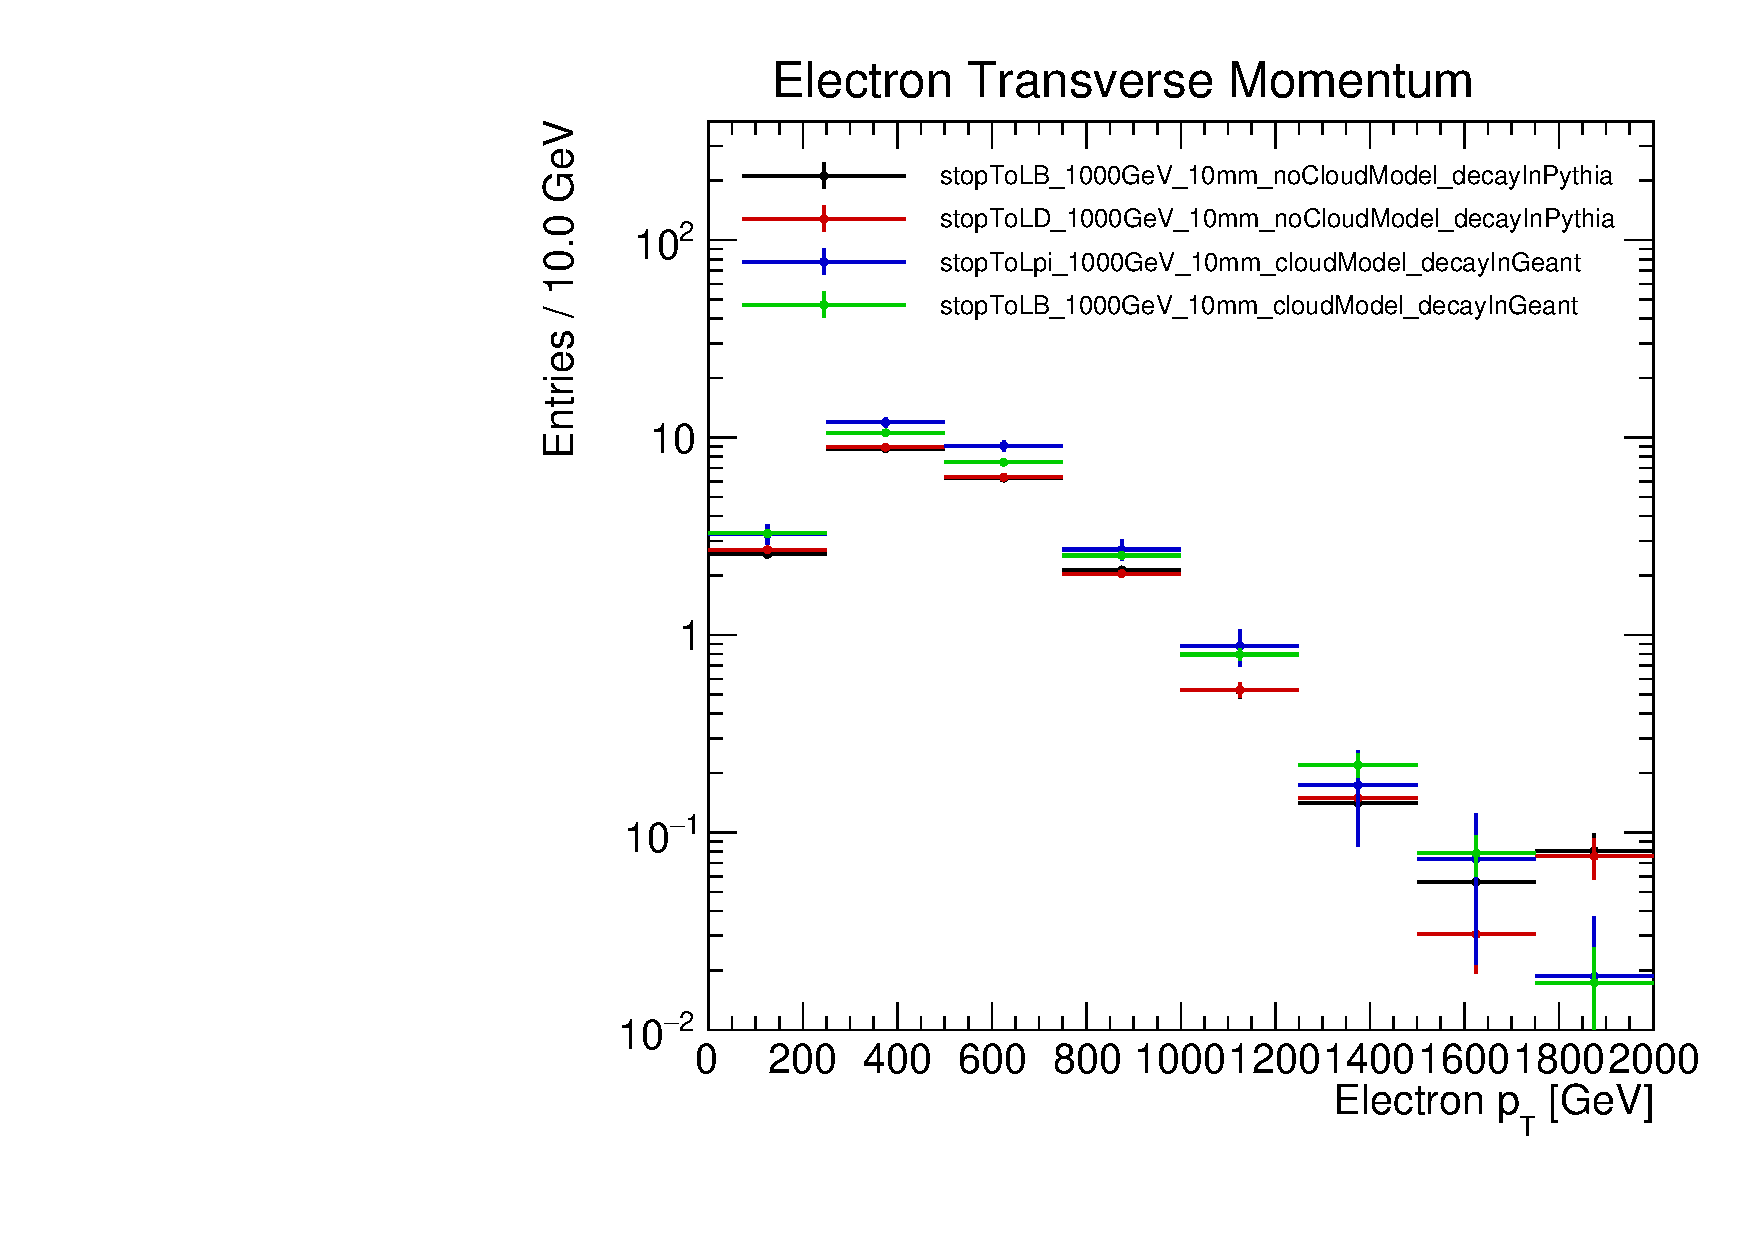
\includegraphics[width=0.34\textwidth]{figures/r_hadrons/eeSR_ePt_1000GeV_10mm.pdf}
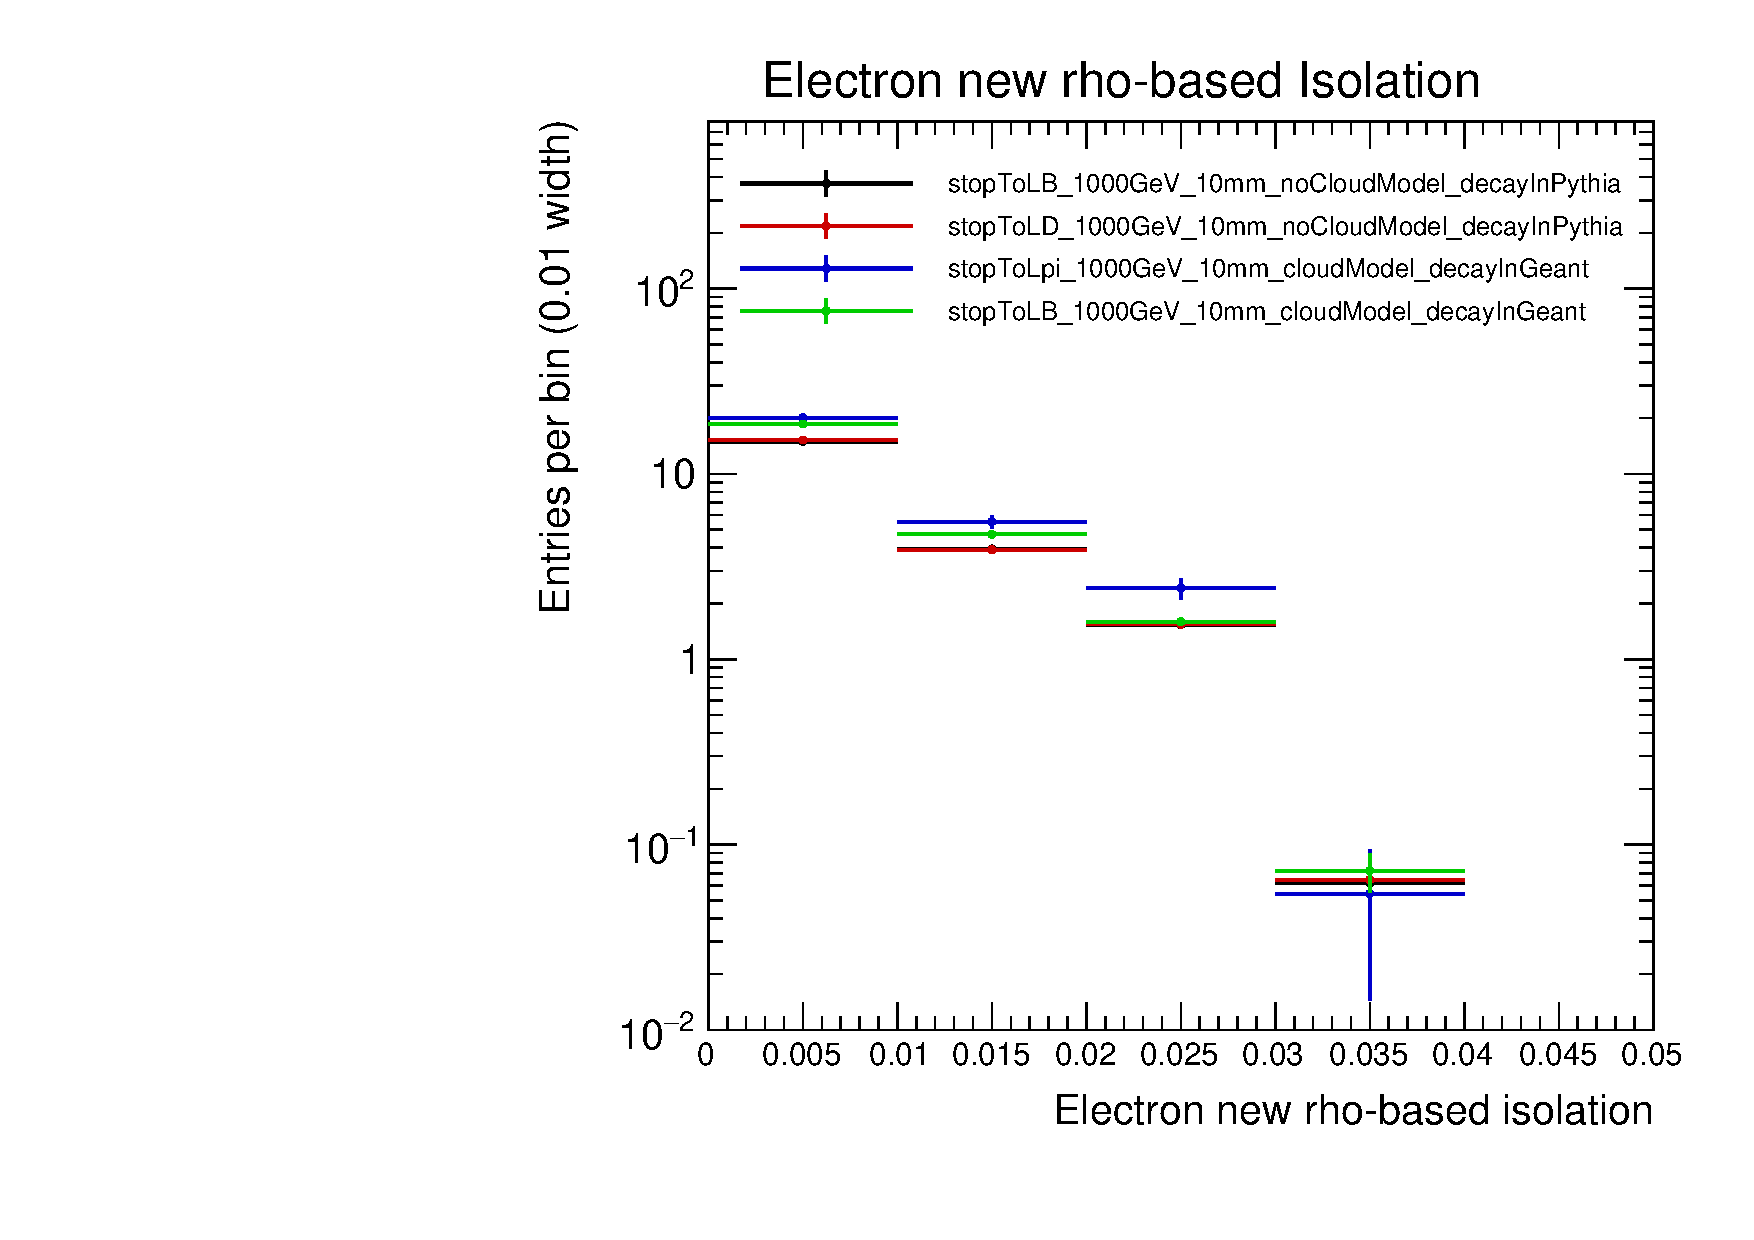
\includegraphics[width=0.34\textwidth]{figures/r_hadrons/eeSR_eIso_1000GeV_10mm.pdf}
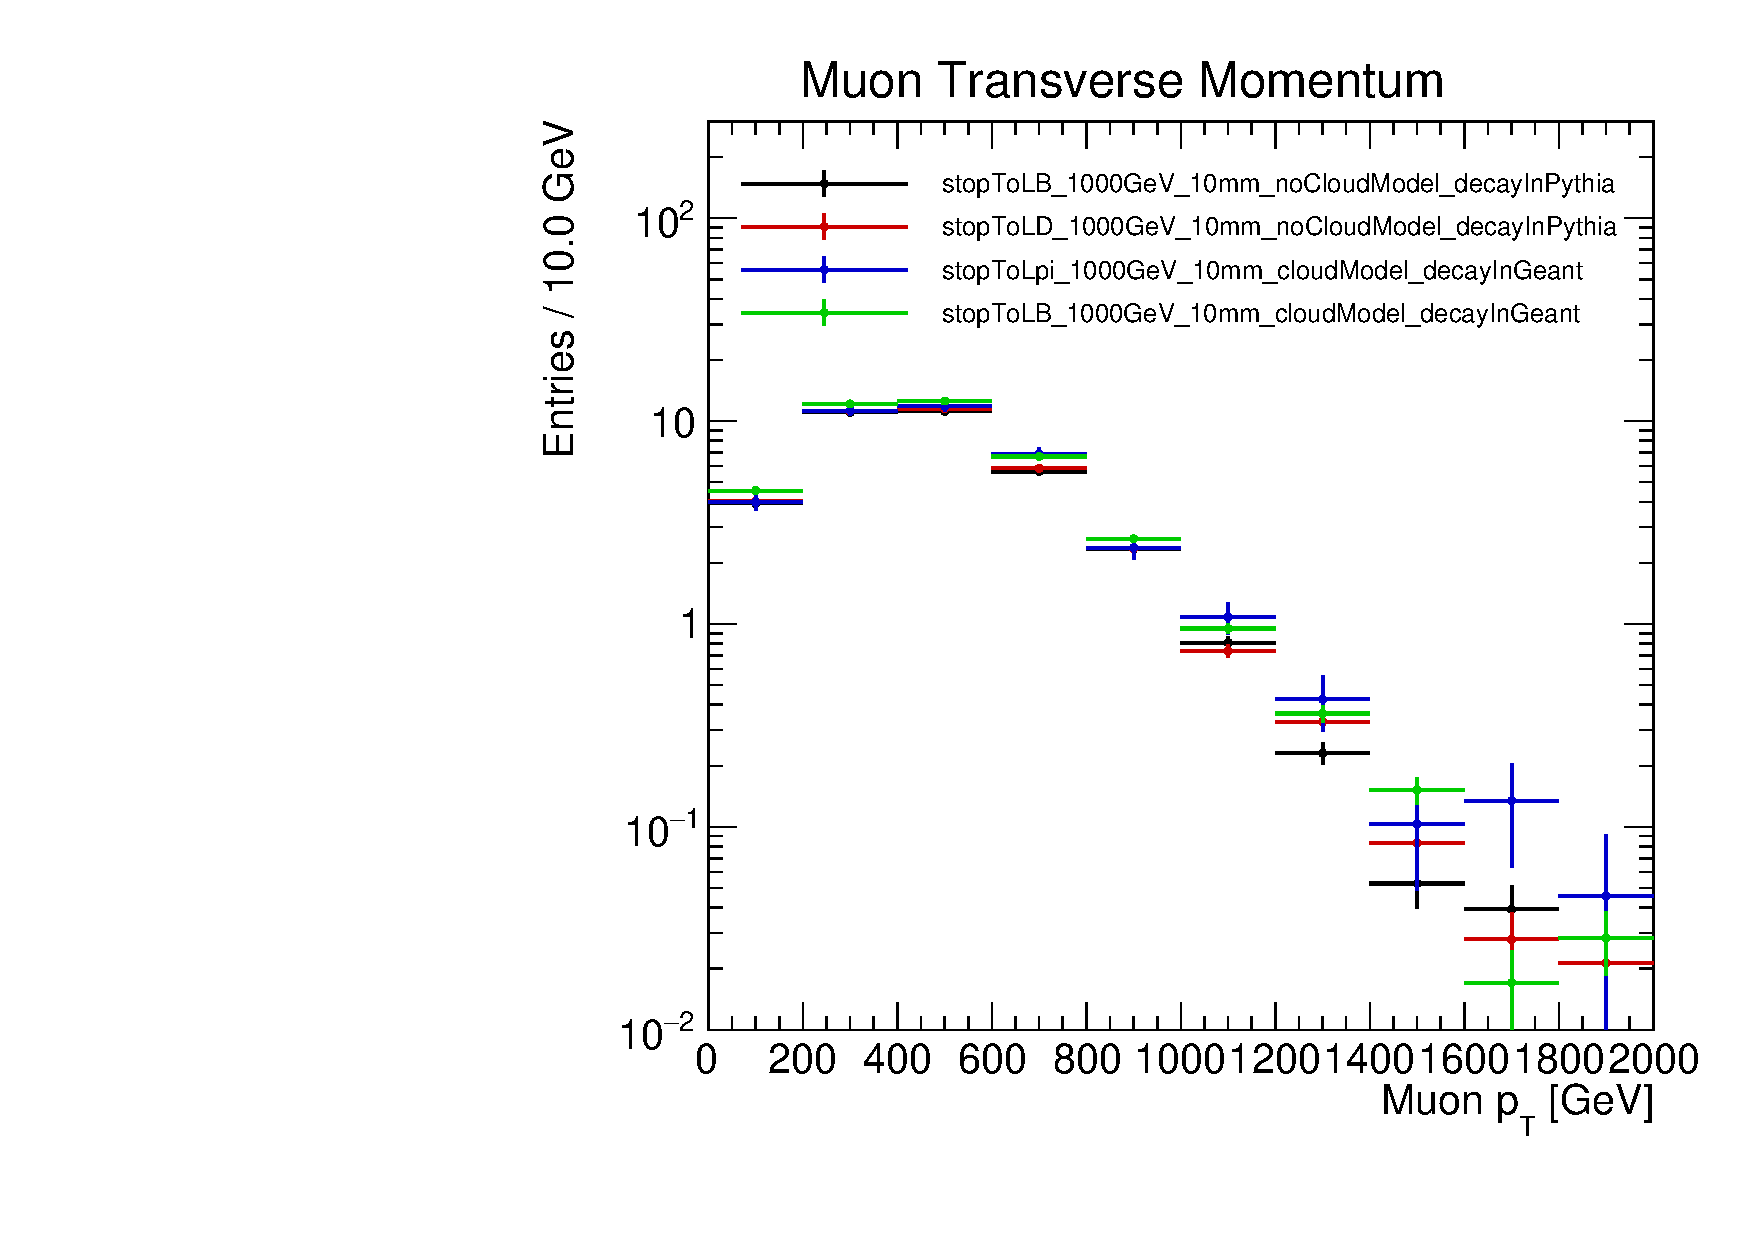
\includegraphics[width=0.34\textwidth]{figures/r_hadrons/mumuSR_muPt_1000GeV_10mm.pdf}
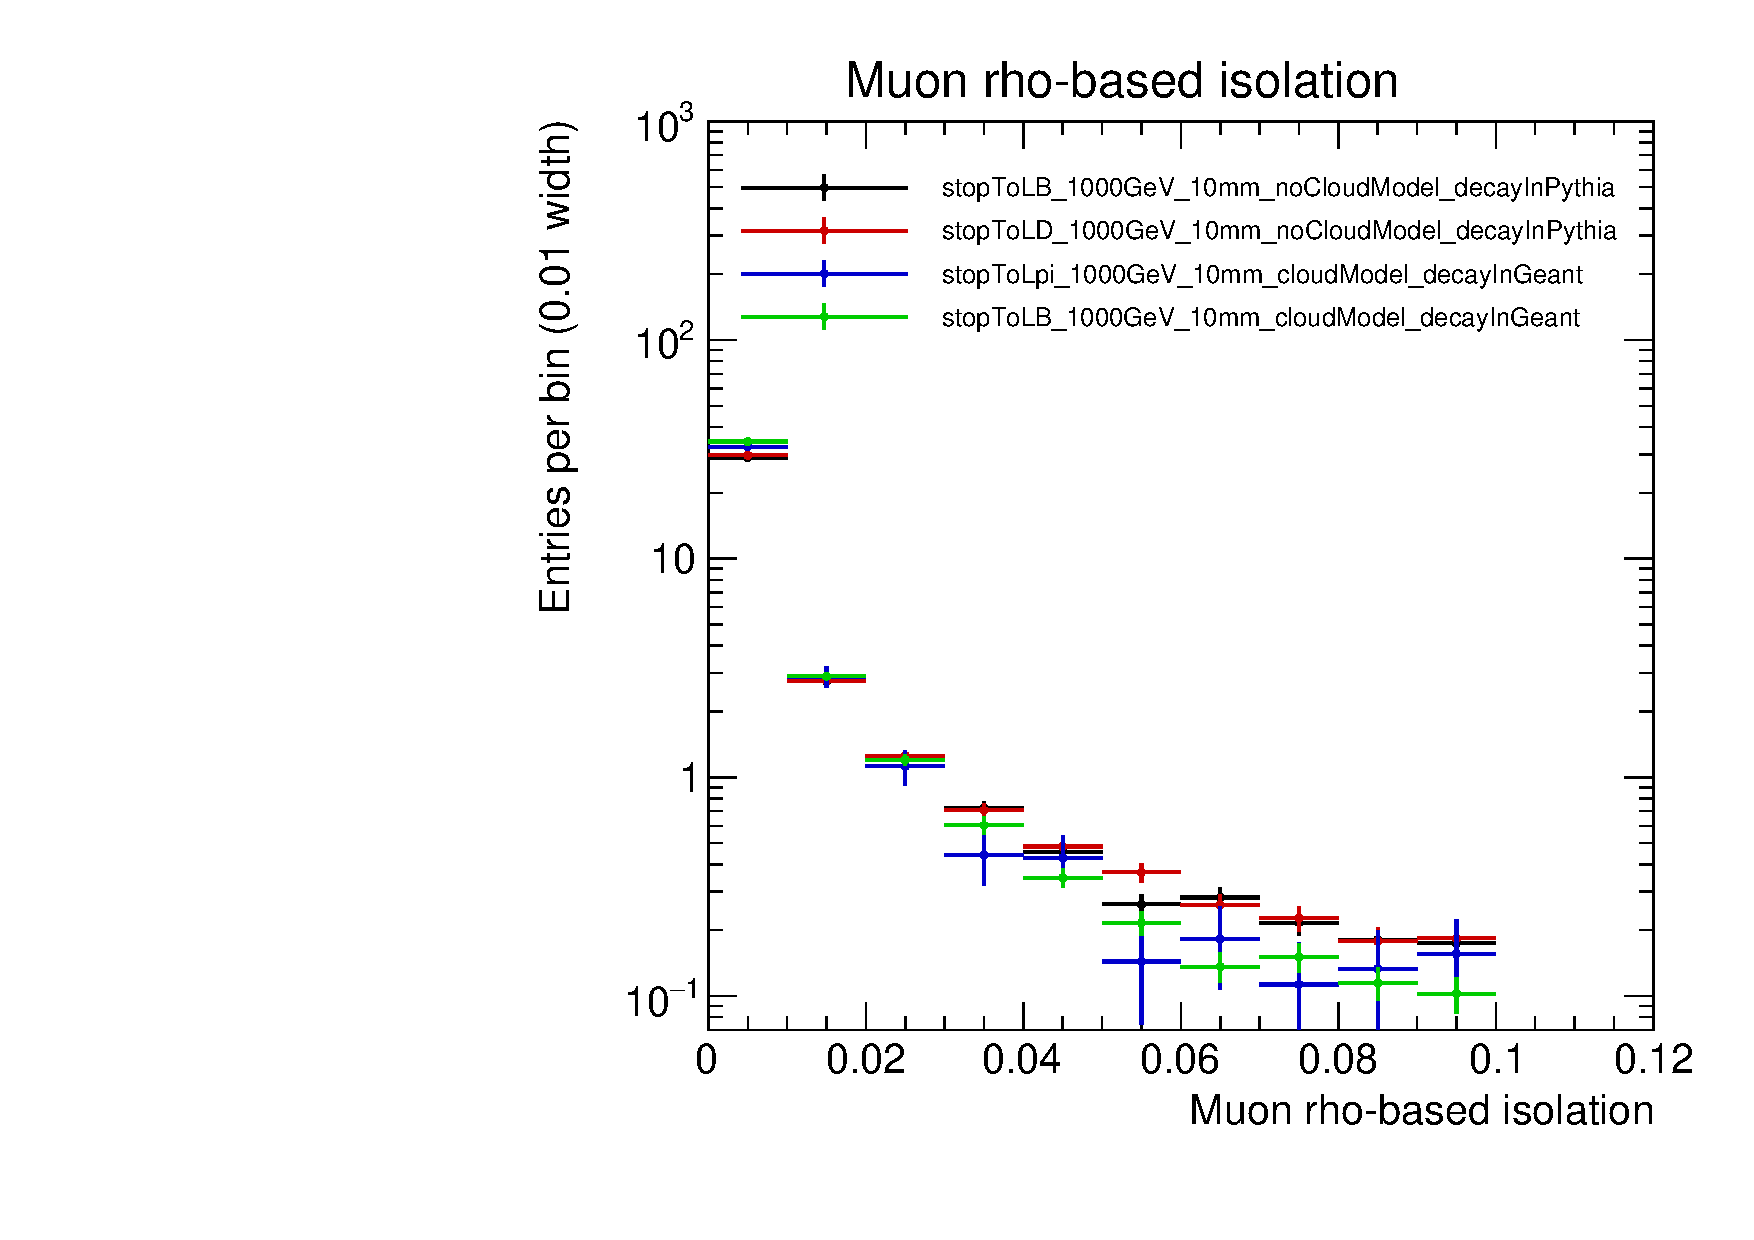
\includegraphics[width=0.34\textwidth]{figures/r_hadrons/mumuSR_muIso_1000GeV_10mm.pdf}
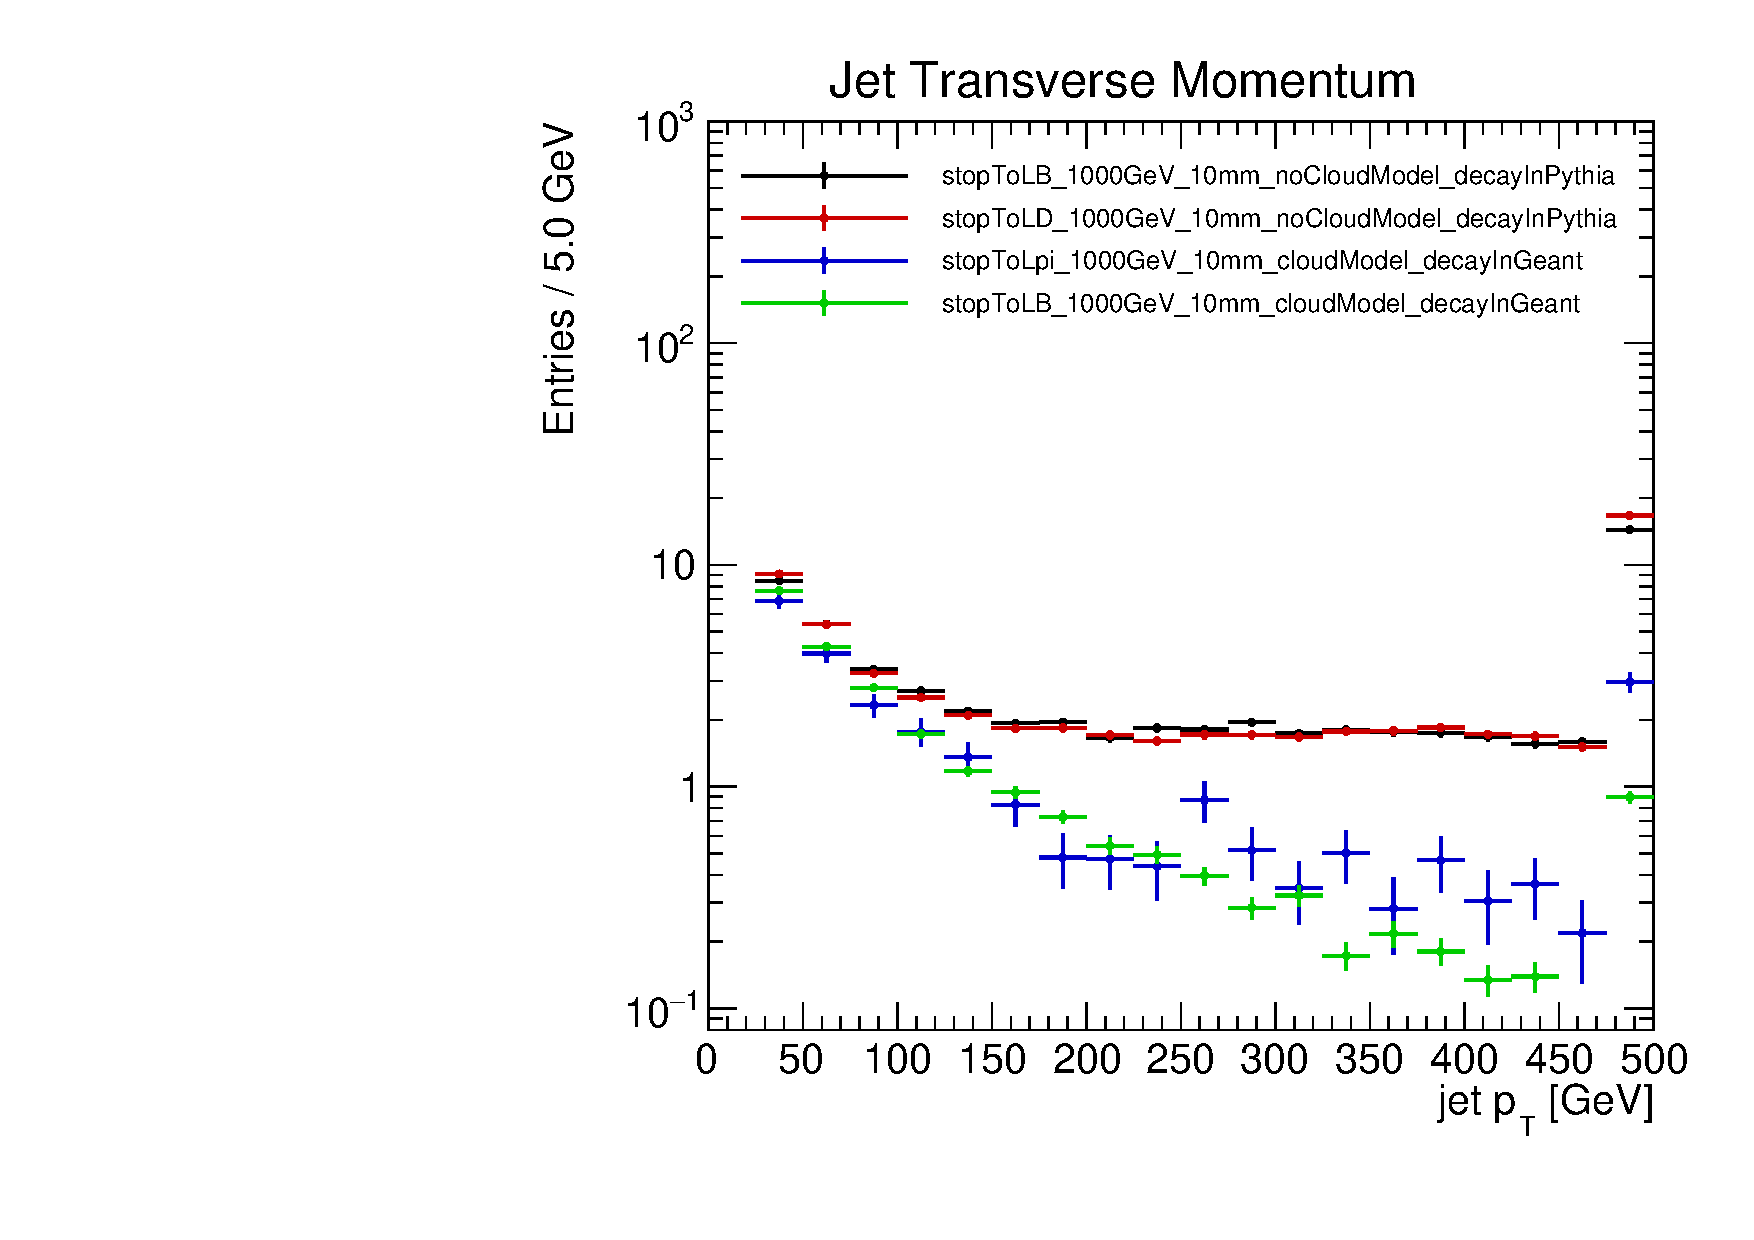
\includegraphics[width=0.34\textwidth]{figures/r_hadrons/mumuSR_jetPt_1000GeV_10mm.pdf}
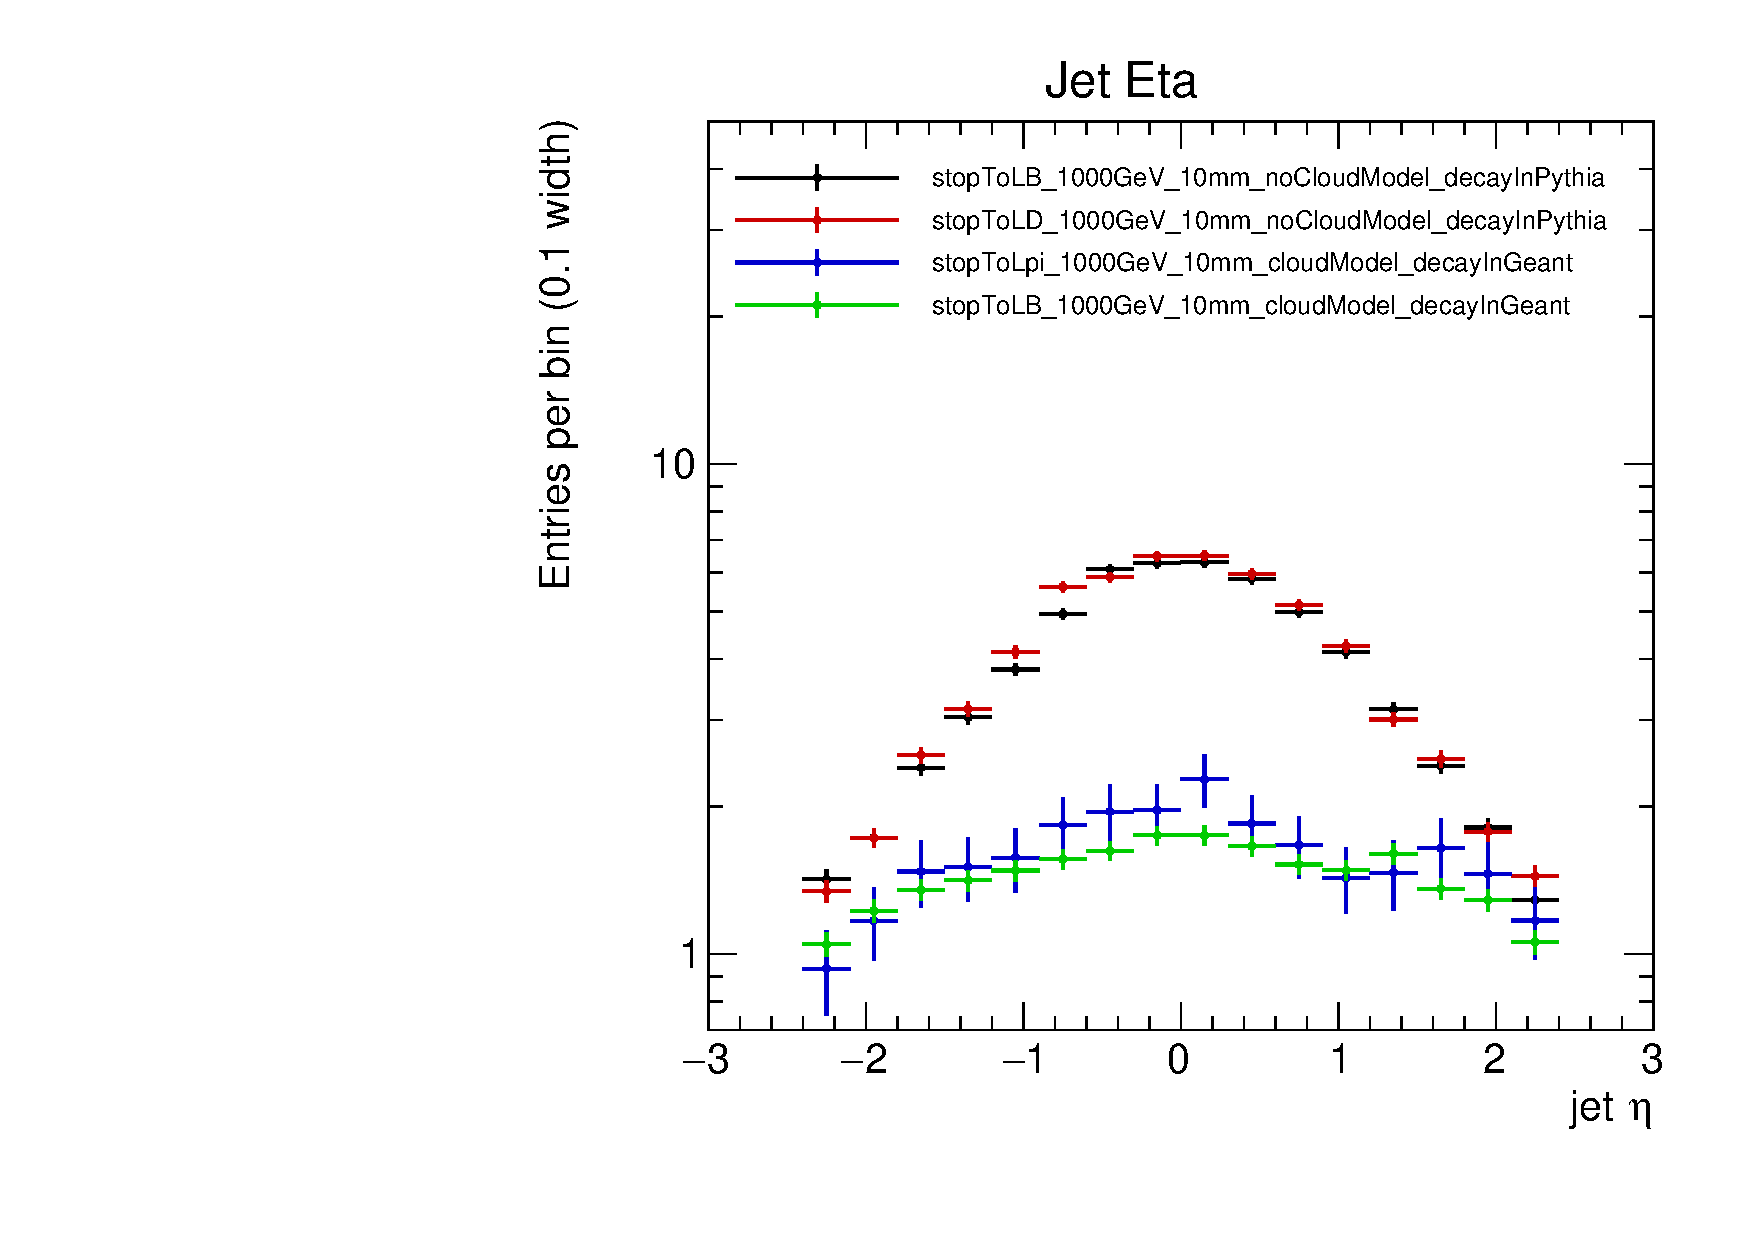
\includegraphics[width=0.34\textwidth]{figures/r_hadrons/mumuSR_jetEta_1000GeV_10mm.pdf}
\caption{
Kinematic distributions of electrons in the $\Pe\Pe$ signal region (top), muons in the $\Pgm\Pgm$ signal region (middle), and jets in the $\Pgm\Pgm$ signal region (bottom) for four signal samples in which the top squark mass and proper decay length are 1000\GeV and 1\cm. In the sample corresponding to the black (red) curves, R-hadron material interactions are not modeled, but the top squark decay is performed in \PYTHIA and the resulting b (d) quark produces a jet. In the samples corresponding to the blue and green curves, the R-hadron material interactions and decay are modeled with \GEANTfour. In the sample corresponding to the blue curves, the R-hadron decays to a lepton and a neutral pion, and in the sample corresponding to the green curves, the R-hadron decays to a lepton and a non-physical final-state quark.  In each plot, the rightmost bin contains overflow entries.
}
\label{r_hadrons_sr}
\end{figure}